\chapter{Introduction}
\label{chap:Intro}
\textit{The first chapter introduces the subject of visual analytics in general and then goes on to introduce visual analytics in the context of public health and epidemiology. We will delve into the literature around this subject and then we will espouse our own motivations in creating a generalizable public health data visual platform}
\vfill
\minitoc
\newpage
\renewcommand{\baselinestretch}{1.80}\normalsize
Visual analytics tools are used to synthesize information and glean insight from massive, dynamic, ambiguous and often conflicting data. Visual Analytics (VA) is often referred to as a means for dealing with complex, large information sources that require human judgment to identify the expected and discover the unexpected. It is a multidisciplinary field whose core areas are analytical reasoning techniques, visual representation and interaction techniques, data representations and transformations as well as production, presentation and dissemination \cite{thomas2006visual}. 

Analytic reasoning techniques enable users to get deep insights which 	support assessment, planning and decision making. It also allows users to assimilate large amounts of information at once \cite{cook2005illuminating}. In a healthcare setting expected outcomes include more efficient and effective clinical performance monitoring and improvement as well as improved modelling of patient flow and management. Additionally, one can expect increased quality of care, improved safety and efficiency and better support for clinical costing and resource coordination. It can also lead to better planned growth and competitive advantage [cite 3].

%use later when need images
%\begin{figure}[!ht] 
%\centering
%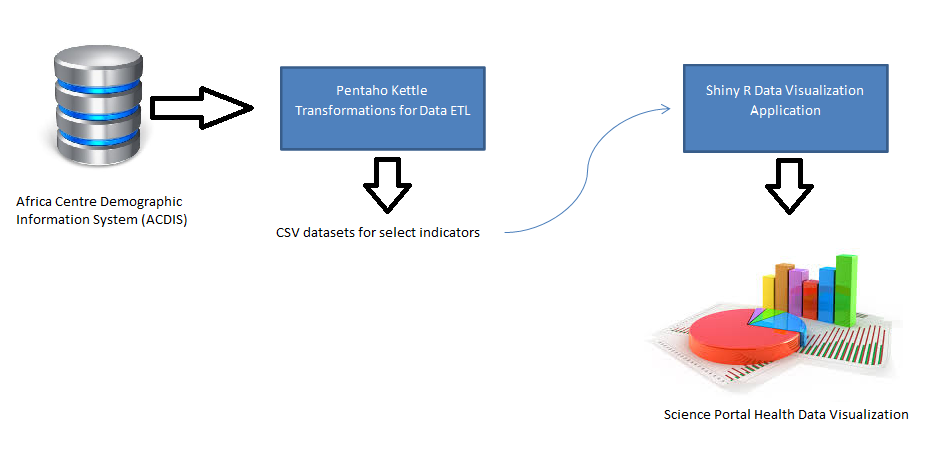
\includegraphics[scale=0.4]{./Chapter1/images/img1}% [width=6in, height=4in]{our}
%\caption{Scientific Portal Solution }
%\label{fig1}
%\end{figure}

VA is referred to as “the science of analytical reasoning facilitated by interactive visual interfaces”. Map based community health visualizations have provided a comprehensive and powerful interface for scientists and policy makers to visualize health care quality, public health outcomes and access to care. This has helped in making evidence-based decisions about improving healthcare [cite 4-7]
 
Multi-panel graphs have also been used to good effect in a graphical tool for epidemiologicalstudies to reveal the distribution of an outcome by time and age simultaneously [cite 8].

The growth of surveillance systems in both quantity of data and variety of outcomes is likely to necessitate constant innovations in data processing, synthesis, and communication [cite 8]
Therefore, techniques to support production, presentation and dissemination of analytic results will allow us to communicate the information in the appropriate context to a variety of audiences.


%\begin{algorithm}[ht]
%%\SetKwInOut{Input}{input}\SetKwInOut{Output}{output}
%%\dontprintsemicolon
%\SetKwInOut{Input}{input}\SetKwInOut{Output}{output}
%\Input{$IndicatorFile\ eIndic,\ Indicator\ nIndic$}
%\Output{$IndicatorFile\ oIndic$}
%\BlankLine
%\Begin {
%\BlankLine
%    $pIndic \longleftarrow eIndic \times nIndic$\;
%    $newNode \longleftarrow new\, internalNode()$\;
%
%    \BlankLine
%		\If{$pIndic.label = \emptyset$}	{
%		   \BlankLine
%		   $pIndic.label \longleftarrow NULL$\;
%		   \BlankLine
%        }
%         \BlankLine
%   		\If{$pIndic.label \neq pIndic.newIndic$}	{
%		   \BlankLine
%		   $nwIndic \longleftarrow createTrunObj()$\;
%		   \BlankLine
%        }   
%    
%%    \For{$i\leftarrow midpoint$ \KwTo $m-1$}{
%%    	\BlankLine
%%    	$newLeaf[j] \longleftarrow leaf.remove(i)$\;
%%    	$j++$ \;
%%    	\BlankLine
%%    }
%    \BlankLine
%	$oIndic \longleftarrow WriteFile(nwIndic)$
%	\BlankLine
%    \BlankLine
%}
%\caption{InsertIndicator \label{IRsplit}}
%\end{algorithm}


\section{Problem Statement}
One critical requirement for successful public health surveillance is the ability to analyse and present data so that it is understandable to a range of public health stakeholders. In public health, VA can be viewed as the bridge between the availability of surveillance data in database architectures and useful information derived from this available data [cite 9].

INDEPTH Health and Demographic Surveillance Sites (HDSS's) deal with complex longitudinal data and, as a result, knowledge transfer to stakeholders is challenging. Better visualisation of this data is therefore required in order for potential scientific users to maximise exploratory data analysis and hypothesis generation. It would also aid decision-makers and the society at large to visualise this information in terms understandable by them. Such a visualization tool will also improve field work research activities by providing summary data of operational progress, e.g. fieldwork data collection progress, data entry progress, or other parameters such as data quality. This will serve to improve operational decision making and data quality. However, datasets at HDSS sites are normally under-visualised. These HDSS sites currently have no generalizable framework for implementing a data visualization platform to be used at these sites.

\section{Motivation}

The current under-visualization of HDSS datasets shows little promise of improvement in a harmonised way (across multiple sites) unless specific research efforts are directed towards finding a generalizable solution for delivering interactive visualizations, supporting exploratory analyses and real-time displays of operational progress. Furthermore, there is a paucity of research specifically on the technologies and tools which can be used to create such a data visualization [cite 10].